\documentclass{standalone}

\usepackage{tikz,tikz-3dplot,pgfplots,xcolor}
\usetikzlibrary{arrows.meta,calc}

%\pgfplotsset{compat=1.18} 
\definecolor{gray0}{rgb}{0.98,0.98,0.98}
\definecolor{gray1}{rgb}{0.8,0.8,0.8}
\definecolor{gray2}{rgb}{0.7,0.7,0.7}

\begin{document}

  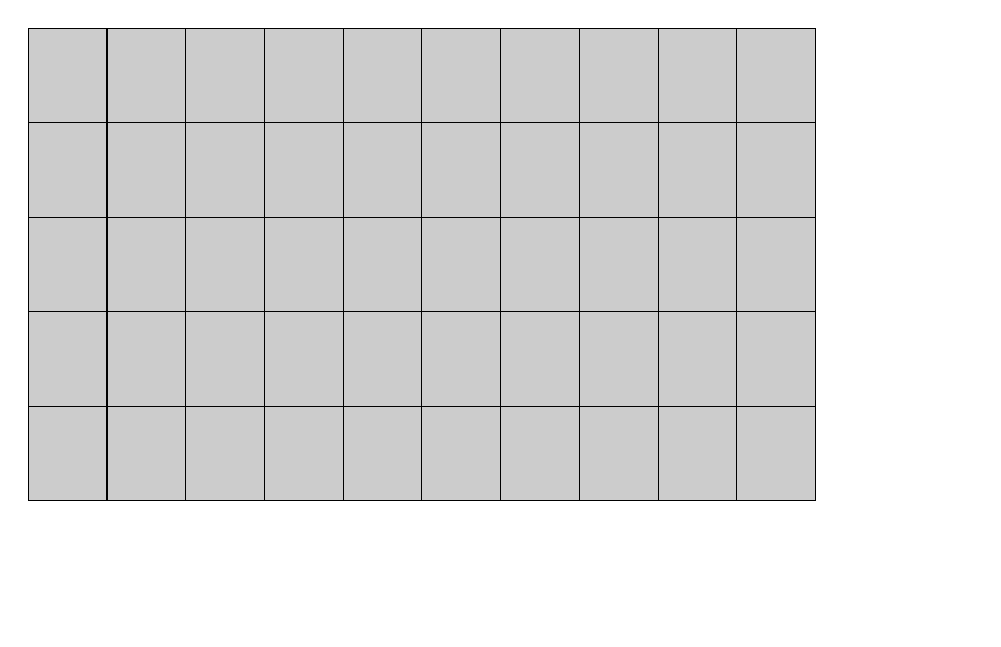
\begin{tikzpicture}[>=Latex]

    \path (0,-1.5) rectangle (12,6);
    \path[fill=gray1] (0,0) rectangle (10,6);
    \foreach \x in {0,...,10}{
      \draw (\x,0) --++ (0,6);
    }
    \foreach \x in {0,...,5}{
      \draw (0,\x*1.2) --++ (10,0);
    }

  \end{tikzpicture}
\end{document}  